\documentclass[tikz,border=7pt]{standalone}
\usepackage[T1]{fontenc}
\usepackage{lmodern}
\usepackage{helvet}
\renewcommand{\familydefault}{\sfdefault}
\usepackage{amsmath}
\usepackage{xcolor}
\usepackage{tikz}
\usetikzlibrary{
  arrows.meta,
  positioning,
  calc,
  fit,
  shapes.geometric,
  shapes.symbols,
  backgrounds,
  decorations.pathreplacing,
  decorations.pathmorphing,
}

\definecolor{slate}{HTML}{334155}
\definecolor{teal}{HTML}{0D9488}
\definecolor{amber}{HTML}{D97706}
\definecolor{rose}{HTML}{E11D48}
\definecolor{muted}{HTML}{64748B}
\definecolor{line}{HTML}{94A3B8}
\definecolor{pagebg}{HTML}{F8FAFC}
\definecolor{card}{HTML}{FFFFFF}
\definecolor{lightteal}{HTML}{CCFBF1}
\definecolor{lightamber}{HTML}{FEF3C7}
\definecolor{lightrose}{HTML}{FFE4E6}
\definecolor{lightslate}{HTML}{E2E8F0}
\definecolor{blueink}{HTML}{2563EB}
\definecolor{bluewash}{HTML}{DBEAFE}
\definecolor{greenink}{HTML}{16A34A}
\definecolor{greenwash}{HTML}{DCFCE7}
\definecolor{pinkink}{HTML}{DB2777}
\definecolor{pinkwash}{HTML}{FCE7F3}

\tikzset{
  >=Stealth,
  font=\sffamily\scriptsize,
  every node/.append style={text=slate},
  title/.style={font=\sffamily\bfseries\small, text=slate, anchor=west},
  note/.style={font=\sffamily\tiny, text=muted, align=left},
  label/.style={font=\sffamily\tiny, text=muted},
  chip/.style={
    draw=#1,
    fill=#1!12,
    rounded corners=2pt,
    inner sep=2.5pt,
    font=\sffamily\tiny\bfseries,
    text=slate,
  },
  decision/.style={
    shape=diamond,
    aspect=2.1,
    draw=teal,
    fill=lightteal,
    inner sep=1.5pt,
    align=center,
    font=\sffamily\tiny,
    text=slate,
  },
  pics/person/.style 2 args={
    code={
      \fill[#1] (0,0.92) circle (0.18);
      \fill[#1]
        (-0.26,0.68)
        .. controls (-0.34,0.42) and (-0.30,0.18) .. (-0.22,0.02)
        -- (0.22,0.02)
        .. controls (0.30,0.18) and (0.34,0.42) .. (0.26,0.68)
        -- cycle;
      \node[font=\sffamily\tiny\bfseries, text=#1, anchor=north] at (0,-0.08) {#2};
    }
  },
  pics/disk/.style={
    code={
      \fill[lightslate] (0,-0.04) ellipse (0.28 and 0.10);
      \fill[slate] (-0.28,-0.04) rectangle (0.28,0.12);
      \fill[slate] (0,0.12) ellipse (0.28 and 0.10);
      \fill[card] (0,0.14) ellipse (0.11 and 0.04);
    }
  },
}

\begin{document}
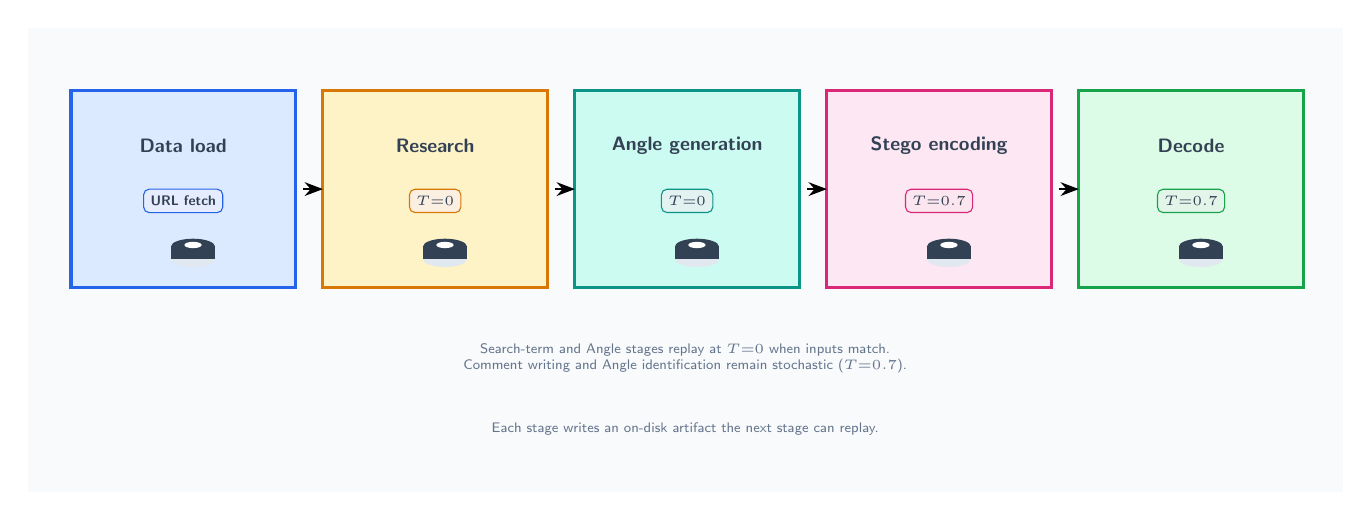
\begin{tikzpicture}[x=1cm,y=1cm]
  \fill[pagebg] (-0.25,-0.55) rectangle (16.45,5.35);

  \foreach \i/\title/\fillc/\drawc/\temp/\x in {
    1/Data load/bluewash/blueink/URL fetch/0.3,
    2/Research/lightamber/amber/$T{=}0$/3.5,
    3/Angle generation/lightteal/teal/$T{=}0$/6.7,
    4/Stego encoding/pinkwash/pinkink/$T{=}0.7$/9.9,
    5/Decode/greenwash/greenink/$T{=}0.7$/13.1} {
    \fill[\fillc] (\x,2.05) rectangle (\x+2.85,4.55);
    \draw[\drawc, line width=1.1pt] (\x,2.05) rectangle (\x+2.85,4.55);
    \node[font=\sffamily\bfseries\scriptsize, align=center, text width=2.5cm] at (\x+1.425,3.85) {\title};
    \node[chip=\drawc] at (\x+1.425,3.15) {\temp};
    \begin{scope}[shift={(\x+1.55,2.45)}]
      \pic {disk};
    \end{scope}
  }
  \foreach \x in {3.25,6.45,9.65,12.85} {
    \draw[thick, ->] (\x,3.30) -- (\x+0.25,3.30);
  }

  \node[note, align=center, text width=15.5cm] at (8.1,1.15) {%
    Search-term and Angle stages replay at $T{=}0$ when inputs match.\\
    Comment writing and Angle identification remain stochastic ($T{=}0.7$).};
  \node[label] at (8.1,0.25) {Each stage writes an on-disk artifact the next stage can replay.};
\end{tikzpicture}
\end{document}
